%%%%%%%%%%%%%%%%%%%%%%%%%%%%%%%%%%%%%%%%%%%%%%%%%%%%%%%%
%                IAML 2020 Assignment 1                %
%                                                      %
%                                                      %
% Authors: Oisin Mac Aodha and Octave Mariotti         %
% Using template from: Michael P. J. Camilleri and     %
% Traiko Dinev.                                        %
%                                                      %
% Based on the Cleese Assignment Template for Students %
% from http://www.LaTeXTemplates.com.                  %
%                                                      %
% Original Author: Vel (vel@LaTeXTemplates.com)        %
%                                                      %
% License:                                             %
% CC BY-NC-SA 3.0                                      %
% (http://creativecommons.org/licenses/by-nc-sa/3.0/)  %
%                                                      %
%%%%%%%%%%%%%%%%%%%%%%%%%%%%%%%%%%%%%%%%%%%%%%%%%%%%%%%%

%--------------------------------------------------------
%   IMPORTANT: Do not touch anything in this part
\documentclass[12pt]{article}
\input{style.tex}



% Options for Formatting Output

\global\setbool{clearon}{true} %
\global\setbool{authoron}{true} %



\newcommand{\assignmentQuestionName}{Question}
\newcommand{\assignmentTitle}{Assignment\ \#1}

\newcommand{\assignmentClass}{IAML -- INFR10069 (LEVEL 10)}

\newcommand{\assignmentWarning}{NO LATE SUBMISSIONS} % 
\newcommand{\assignmentDueDate}{Tues,\ October\ 20,\ 2020 @ 16:00}
%--------------------------------------------------------


%%%%%%%%%%%%%%%%%%%%%%%%%%%%%%%%%%%%%%%%%%%%%%%%%%%%%%%
%
% NOTE: YOU NEED TO ENTER YOUR STUDENT ID BELOW.
%
%%%%%%%%%%%%%%%%%%%%%%%%%%%%%%%%%%%%%%%%%%%%%%%%%%%%%%%%
%--------------------------------------------------------
% IMPORTANT: Specify your Student ID below. You will need to uncomment the line, else compilation will fail. Make sure to specify your student ID correctly, otherwise we may not be able to identify your work and you will be marked as missing.
\newcommand{\assignmentAuthorName}{s1720422}
%--------------------------------------------------------



\begin{document}
\maketitle
\thispagestyle{empty}







%%%%%%%%%%%%%%%%%%%%%%%%%%%%%%%%%%%%%%%%%%%%%%%%%%%%%%%%%%%%%%%%%%%%%%%%%%%%%%
%============================================================================%
%%%%%%%%%%%%%%%%%%%%%%%%%%%%%%%%%%%%%%%%%%%%%%%%%%%%%%%%%%%%%%%%%%%%%%%%%%%%%%
\clearpage

\begin{question}{(22 total points) Linear Regression}

\questiontext{In this question we will fit linear regression models to data.}



%
%
\begin{subquestion}{(3 points) Describe the main properties of the data, focusing on the size, data ranges, and data types.   
}


\begin{answerbox}{10em}
The data set is represented by a 50 by 2 pandas data frame. It contains 50 data points and 2 columns for the attributes 'revision\_time' and 'exam\_score'. These attributes are both of the float64 data type. The float values for 'revision\_time' vary from a minimum of 2.72 to a maximum of 48.0. The float values for 'exam\_score' vary from a minimum of 49.9 to a maximum of 94.9. 
\end{answerbox}



\end{subquestion}




%
%
\begin{subquestion}{(3 points) Fit a linear model to the data so that we can predict \texttt{exam\_score} from \texttt{revision\_time}. 
Report the estimated model parameters $\mathbf{w}$. 
Describe what the parameters represent for this 1D data. 
For this part, you should use the sklearn implementation of \href{https://scikit-learn.org/0.19/modules/generated/sklearn.linear_model.LinearRegression.html}{Linear Regression}.\\
\hint{By default in sklearn \texttt{fit\_intercept = True}. Instead, set \texttt{fit\_intercept = False} and pre-pend $1$ to each value of $x_i$ yourself to create $\boldsymbol{\phi}(x_i) = [1, x_i]$. 
}
}


\begin{answerbox}{10em}
The estimated model parameters are $w = [17.9, 1.44]$ to 3 s.f. The values of $w$ represent the estimated weight coefficients for the linear regression model. In this case the first value 17.9 represents the y-intercept of the line and the value of 1.44 represents the coefficient for the 'revision\_time' attribute.  
\end{answerbox}



\end{subquestion}



%
%
\begin{subquestion}{(3 points) Display the fitted linear model and the input data on the same plot.
}


\begin{answerbox}{35em}
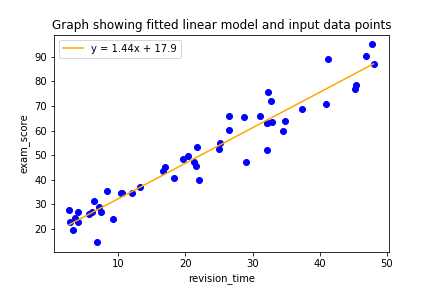
\includegraphics[width = 1.0\textwidth]{q1_c.png}
\end{answerbox}



\end{subquestion}



%
%
\begin{subquestion}{(3 points) Instead of using sklearn, implement the closed-form solution for fitting a linear regression model yourself using numpy array operations.  
Report your code in the answer box.
It should only take a few lines (i.e. <5).\\ 
\hint{Only report the relevant lines for estimating $\mathbf{w}$ e.g. we do not need to see the data loading code. You can write the code in the answer box directly or paste in an image of it. }
}


\begin{answerbox}{20em}
x\_new contains the column of 1's and the column of revision\_time values. The code used to calculate the weights is as follows:
\begin {verbatim}
x_new = np.ones((50, 2))
x_new[:,1] = r_part1['revision_time']
w = np.dot(x_new.T, x_new)
w1 = np.dot(np.linalg.pinv(w), np.dot(x_new.T, y))
print(w1)
\end {verbatim}
\end{answerbox}



\end{subquestion}



%
%
\begin{subquestion}{(3 points) Mean Squared Error (MSE) is a common metric used for evaluating the performance of regression models. 
Write out the expression for MSE and list one of its limitations. \\
\hint{For notation, you can use $y$ for the ground truth quantity and $\hat{y}$ (\texttt{\$\textbackslash{}hat\{y\}\$} in latex) in place of the model prediction.}
}


\begin{answerbox}{10em}
$MSE = \frac{1}{n}\sum\limits_{i=1}^n(y_i-\hat{y_i})^2$ where $n$ is the number of data point instances, $\hat{y_i}$ is the predicted value for instance $i$, and $y_i$ is the ground truth value for instance $i$.
A limitation of using MSE is that it's sensitive to outliers and gives a lot of weight to them compared to other methods.
\end{answerbox}



\end{subquestion}


 
%
%
\begin{subquestion}{(3 points) Our next step will be to evaluate the performance of the fitted models using Mean Squared Error (MSE). 
Report the MSE of the data in \texttt{regression\_part1.csv} for your prediction of \texttt{exam\_score}.
You should report the MSE for the linear model fitted using sklearn and the model resulting from your closed-form solution. 
Comment on any differences in their performance. 
}


\begin{answerbox}{10em}
Linear regression model results are show below:
\begin{center}
\begin{tabular}{c|c}
 \hline
 Solution & MSE \\ \hline
 sklearn & 30.9854726145413 \\
 closed-form & 30.98547261454128 \\
 \hline
\end{tabular}
\end{center}
All s.f have been displayed as the sklearn version has rounded up the result whereas the closed-form version hasn't. The performance difference is minimal.
\end{answerbox}



\end{subquestion}




%
%
\begin{subquestion}{(4 points) Assume that the optimal value of $w_0$ is $20$, it is not but let's assume so for now. 
Create a plot where you vary $w_1$ from $-2$ to $+2$ on the horizontal axis, and report the Mean Squared Error on the vertical axis for each setting of $\mathbf{w} = [w_0, w_1]$ across the dataset. 
Describe the resulting plot. Where is its minimum? Is this value to be expected?\\ 
\hint{You can try 100 values of $w_1$ i.e. \texttt{w1 = np.linspace(-2,2, 100)}.}
}


\begin{answerbox}{35em}
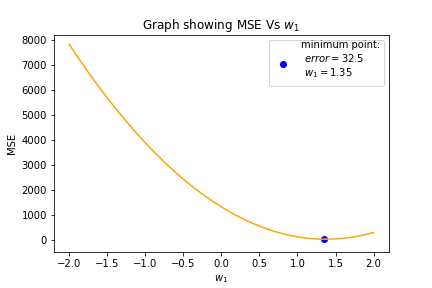
\includegraphics[width = 1\textwidth]{q1_g.png}

The resulting plot shows that as the coefficient $w_1$ increases, the MSE reduces significantly until the minimum point is reached(indicated in blue above). A minimum of $w_1 = 1.35$ is expected as it isn't too far away from 1.44 which was the $w_1$ value the classifier generated from the data set. The reason this $w_1$ value is lower is due to us making the assumption that the y-intercept, $w_0$ is 20. This changes the value of the optimal slope($w_1$) that gets fitted to the model. 

\end{answerbox}



\end{subquestion}


 
\end{question}





%%%%%%%%%%%%%%%%%%%%%%%%%%%%%%%%%%%%%%%%%%%%%%%%%%%%%%%%%%%%%%%%%%%%%%%%%%%%%%
%============================================================================%
%%%%%%%%%%%%%%%%%%%%%%%%%%%%%%%%%%%%%%%%%%%%%%%%%%%%%%%%%%%%%%%%%%%%%%%%%%%%%%
\clearpage



\begin{question}{(18 total points) Nonlinear Regression}

\questiontext{In this question we will tackle regression using basis functions.}




%
%
\begin{subquestion}{(5 points) Fit four different polynomial regression models to the data  by varying the degree of polynomial features used i.e. $M = 1$ to $4$.
For example, $M=3$ means that $\boldsymbol{\phi}(x_i) = [1, x_i, x_i^2, x_i^3]$.
Plot the resulting models on the same plot and also include the input data.\\
\hint{
 You can again use the sklearn implementation of \href{https://scikit-learn.org/0.19/modules/generated/sklearn.linear_model.LinearRegression.html}{Linear Regression} and you can also use \href{https://scikit-learn.org/0.19/modules/generated/sklearn.preprocessing.PolynomialFeatures.html}{PolynomialFeatures} to generate the polynomial features. Again, set \texttt{fit\_intercept = False}.}
}


\begin{answerbox}{35em}
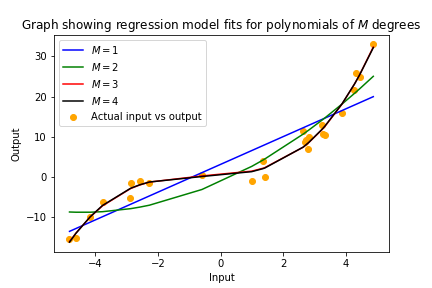
\includegraphics[width = 1\textwidth]{q2.png}
\end{answerbox}



\end{subquestion}


%
%
\begin{subquestion}{(3 points) Create a bar plot where you display the Mean Squared Error of each of the four different polynomial regression models from the previous question.}


\begin{answerbox}{35em}
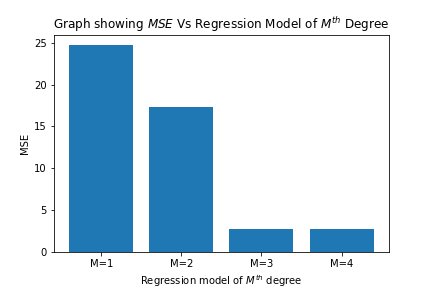
\includegraphics[width = 1.0\textwidth]{q2_b.png}
\end{answerbox}



\end{subquestion}


%
%
\begin{subquestion}{(4 points) Comment on the fit and Mean Squared Error values of the $M=3$ and $M=4$ polynomial regression models. 
Do they result in the same or different performance? 
Based on these results, which model would you choose?}


\begin{answerbox}{15em}
The $MSE$ for the $M=3$ and $M=4$ regression models both round to 2.74 to 3 s.f. The $M=4$ model has a slightly lower MSE of $2.7389...$ however the difference is negligible so the performance would most likely be similar. There are 2 reasons why I would choose the $M=3$ regression model. The first being that the actual input/output scatter plot was shaped like a cubic and the fit for the $M=3$ classifier was ideal. The second reason being that despite the $M = 4$ model producing a similar fit, there is a chance that picking it would result in the overfitting of future data. A model of a higher degree is more flexible and very sensitive. Picking the $M=3$ model is less likely to cause such an issue, so I think it's the sensible choice.
\end{answerbox}



\end{subquestion}



%
%
\begin{subquestion}{(6 points) Instead of using polynomial basis functions, in this final part we will use another type of basis function - radial basis functions (RBF). 
Specifically, we will define $\boldsymbol{\phi}(x_i) = [1, rbf(x_i; c_1, \alpha), rbf(x_i; c_2, \alpha), rbf(x_i; c_3, \alpha), rbf(x_i; c_4, \alpha)]$, where $rbf(x; c, \alpha) =  \exp(-0.5(x-c)^2 / \alpha^2)$ is an RBF kernel with center $c$ and width $\alpha$. Note that in this example, we are using the same width $\alpha$ for each RBF, but different centers for each.\\ 
Let $c_1=-4.0$, $c_2=-2.0$, $c_3=2.0$, and $c_4=4.0$ and plot the resulting nonlinear predictions using the \texttt{regression\_part2.csv} dataset for $\alpha \in \{0.2, 100, 1000\}$. 
You can plot all three results on the same figure.
Comment on the impact of larger or smaller values of $\alpha$.
}


\begin{answerbox}{35em}
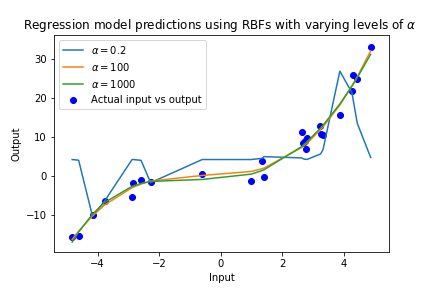
\includegraphics[width = 1.0\textwidth]{q2_d.png}
Upon observation it can be seen that the lower $\alpha$ is, the further away the predicted outputs are from the ground truth outputs. This is because input points with a distance of more than $\alpha$ from the RBF centre points get mapped further away than points which are within the range of the RBF centre points. When $\alpha$ is large, the points are mapped closer together as more points are within range of the RBF features. Having a large $\alpha$ value evidently helps produce predicted outputs closer to the true label values.
\end{answerbox}



\end{subquestion}



\end{question}






%%%%%%%%%%%%%%%%%%%%%%%%%%%%%%%%%%%%%%%%%%%%%%%%%%%%%%%%%%%%%%%%%%%%%%%%%%%%%%
%============================================================================%
%%%%%%%%%%%%%%%%%%%%%%%%%%%%%%%%%%%%%%%%%%%%%%%%%%%%%%%%%%%%%%%%%%%%%%%%%%%%%%
\clearpage


\begin{question}{(26 total points) Decision Trees}

\questiontext{In this question we will train a classifier to predict if a person is smiling or not.}




%
%
\begin{subquestion}{(4 points) Load the data, taking care to separate the target binary class label we want to predict, \texttt{smiling}, from the input attributes. 
Summarise the main properties of both the training and test splits. 
}


\begin{answerbox}{12em}
\begin{center}

\begin{tabular}{c|c|c|c}
 \hline
 Data & Dimensions(row,col) & Type & Contains(per instance) \\ \hline
 X\_train & 4800, 136 & float64 & 68 pairs of (x,y) face features \\
 X\_test & 1200, 136 & float64 & 68 pairs of (x,y) face features \\
 y\_train & 4800, 1 & int64 & 0/1 to show if instance is smiling \\
 y\_test & 1200, 1 & int64 & 0/1 to show if instance is smiling  \\
 \hline
\end{tabular}
\end{center}
The training/test split is approximately a 80/20 split. There are 4800 training instances and 1200 test instances.
\end{answerbox}



\end{subquestion}


%
%
\begin{subquestion}{(4 points) Even though the input attributes are high dimensional, they actually consist of a set of 2D coordinates representing points on the faces of each person in the dataset. 
Create a scatter plot of the average location for each 2D coordinate. One for (i) smiling and (ii) one not smiling faces. 
For instance, in the case of smiling faces, you would average each of the rows where \texttt{smiling = 1}. 
You can plot both on the same figure, but use different colors for each of the two cases. 
Comment on any difference you notice between the two sets of points. \\
\hint{Your plot should contain two faces.}
}
s

\begin{answerbox}{35em}
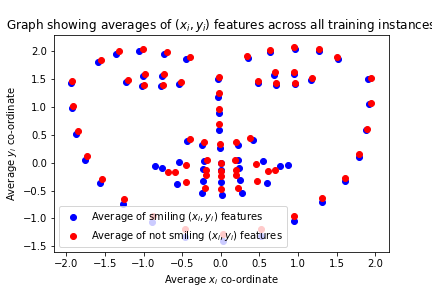
\includegraphics[width = 1.0\textwidth]{q3_b.png}
It can be observed that each pair of smiling $(x,y)$ points are mapped slightly below every $(x,y)$ pair of not smiling points, apart from in the mouth region.

Furthermore, we can see that the smiling $(x,y)$ points in the mouth region span across a larger range of $x$ and $y$ values compared to the not smiling co-ordinates in the mouth region which spans over a smaller range of $x$ and $y$ values. The smiling co-ordinates in this region occupy more space than the not smiling points.
\end{answerbox}



\end{subquestion}


%
%
\begin{subquestion}{(2 points) 
There are different measures that can be used in decision trees when evaluating the quality of a split. 
What measure of purity at a node does the \href{https://scikit-learn.org/0.19/modules/generated/sklearn.tree.DecisionTreeClassifier.html}{DecisionTreeClassifier} in sklearn use for classification by default? 
What is the advantage, if any, of using this measure compared to entropy? 
}


\begin{answerbox}{10em}
The DecisionTreeClassifier in sklearn uses the Gini impurity for classification by default. The advantage of using this metric is that it is computationally less expensive than the calculation for entropy as it doesn't involve calculating logs of values. Therefore it would be ideal to use for data sets with many attributes.
\end{answerbox}



\end{subquestion}


%
%
\begin{subquestion}{(3 points) 
One of the hyper-parameters of a decision tree classifier is the maximum depth of the tree. 
What impact does smaller or larger values of this parameter have? Give one potential problem for small values and two for large values. 
}


\begin{answerbox}{10em}
A samller tree depth would result in less leaves. Therefore, data points are likely to always be classified into the same class. Hence, the model will be inflexible and underfit. A higher depth allows for splits on more attributes, hence increasing the amount of leaves. This allows the pattern in the data to be captured better. However, using a high tree depth could result in the model being overfitted, especially if the tree is grown to full depth as it will fit the training data perfectly. Furthermore, it is computationally expensive when random forests are used.


\end{answerbox}



\end{subquestion}


%
%
\begin{subquestion}{(6 points) 
Train three different decision tree classifiers with a maximum depth of 2, 8, and 20 respectively.
Report the maximum depth, the training accuracy (in \%), and the test accuracy (in \%) for each of the three trees.
Comment on which model is best and why it is best. \\
\hint{Set \texttt{random\_state = 2001} and use the \texttt{predict()} method of the \href{https://scikit-learn.org/0.19/modules/generated/sklearn.tree.DecisionTreeClassifier.html}{DecisionTreeClassifier} so that you do not need to set a threshold on the output predictions.
You can set the maximum depth of the decision tree using the \texttt{max\_depth} hyper-parameter.}
}


\begin{answerbox}{20em}
\begin{center}

\begin{tabular}{c|c|c|c}
 \hline
 Model & Maximum Depth & Training Accuracy(3s.f.) & Test Accuracy(3s.f.)  \\ \hline
 1 & 2 & 79.5\% & 78.2\%  \\
 2 & 8 & 93.4\% &  84.1\% \\
 3 & 20 & 100\% & 81.6\%  \\
 \hline
\end{tabular}
\end{center}
From the results obtained, it can be concluded that model 2 is the best. This is because it obtains a high testing accuracy whilst at the same time not overfitting. Model 3 is overfit as the testing accuracy is less than model 2's despite the 100\% training accuracy.  Model 1 is clearly underfit compared to model 2 as the train and test accuracies are both lower.
\end{answerbox}



\end{subquestion}


%
%
\begin{subquestion}{(5 points) 
Report the names of the top three most important attributes, in order of importance, according to the Gini importance from \href{https://scikit-learn.org/0.19/modules/generated/sklearn.tree.DecisionTreeClassifier.html}{DecisionTreeClassifier}. 
Does the one with the highest importance make sense in the context of this classification task? \\
\hint{Use the trained model with \texttt{max\_depth = 8} and again set  \texttt{random\_state = 2001}.}
}


\begin{answerbox}{10em}
\begin{center}

\begin{tabular}{c|c|c}
 \hline
 Order of Importance & Name of Attribute & Gini importance(3s.f.)  \\ \hline
 1 & $x_50$ & 0.330  \\
 2 & $y_48$ & 0.0900 \\
 3 & $y_29$ & 0.0883  \\
 \hline
\end{tabular}
\end{center}
The $x_{50}$ attribute makes sense to be the most important as when a plot is created for the training $(x_{50},y_{50})$ instances, the points are all centered in the mouth region.
\end{answerbox}



\end{subquestion}



%
%
\begin{subquestion}{(2 points) 
Are there any limitations of the current choice of input attributes used i.e. 2D point locations? If so, name one. 
}


\begin{answerbox}{10em}
There are limitations to using 2D attributes. The main one being that coordinates are continuous variables and can take on an infinite amount of values. Decision trees are known to be very sensitive to changes in input data. If input data is changed sightly, a whole different tree can form. The likelihood of this occurring can be reduced by using attributes which take on a fixed number of values.
\end{answerbox}



\end{subquestion}


\end{question}




%%%%%%%%%%%%%%%%%%%%%%%%%%%%%%%%%%%%%%%%%%%%%%%%%%%%%%%%%%%%%%%%%%%%%%%%%%%%%%
%============================================================================%
%%%%%%%%%%%%%%%%%%%%%%%%%%%%%%%%%%%%%%%%%%%%%%%%%%%%%%%%%%%%%%%%%%%%%%%%%%%%%%
\clearpage


\begin{question}{(14 total points) Evaluating Binary Classifiers}

\questiontext{In this question we will perform performance evaluation of binary classifiers.}




%
%
\begin{subquestion}{(4 points) Report the classification accuracy (in \%) for each of the four different models using the \texttt{gt} attribute as the ground truth class labels. 
Use a threshold of $>= 0.5$ to convert the continuous classifier outputs into binary predictions. 
Which model is the best according to this metric?
What, if any, are the limitations of the above method for computing accuracy and how would you improve it without changing the metric used?
}


\begin{answerbox}{15em}
\begin{center}
\begin{tabular}{c|c}
 \hline
 Classifier & Accuracy  \\ \hline
 alg\_1 & 61.6\%  \\
 alg\_2 & 55\% \\
 alg\_3 & 32.1\%  \\
 alg\_4 & 32.9\%  \\
 \hline
\end{tabular}
\end{center}
According to this metric, alg\_1 is the best model as it has the highest accuracy score. The limitation posed by this metric is that it assumes that the threshold value is optimal. To improve the accuracy, I would test a range of thresholds and select the threshold which optimises the accuracy scores. Alternatively, I would add another threshold in addition to the current one to achieve an improvement.
\end{answerbox}



\end{subquestion}



%
%
\begin{subquestion}{(4 points) Instead of using classification accuracy, report the Area Under the ROC Curve (AUC) for each model. 
Does the model with the best AUC also have the best accuracy? If not, why not?\\
\hint{You can use the  \href{https://scikit-learn.org/0.19/modules/generated/sklearn.metrics.roc\_auc\_score.html}{roc\_auc\_score} function from sklearn.}
}


\begin{answerbox}{15em}
The following AUC values assume the threshold in the previous question hasn't been applied to binarize the predicted class probabilities.
\begin{center}
\begin{tabular}{c|c}
 \hline
 Classifier & AUC (3s.f)  \\ \hline
 alg\_1 & 0.732  \\
 alg\_2 & 0.632 \\
 alg\_3 & 0.0640  \\
 alg\_4 & 0.847  \\
 \hline
\end{tabular}
\end{center}
We can see alg\_4 has the best AUC but not accuracy. AUC represents the best overall performance, so for a specific threshold, alg\_1 may be more accurate(e.g. when $t \geq 0.5$) but generally most of the time alg\_4 outperforms it.
\end{answerbox}



\end{subquestion}



%
%
\begin{subquestion}{(6 points) Plot ROC curves for each of the four models on the same plot.
Comment on the ROC curve for \texttt{alg\_3}?
Is there anything that can be done to improve the performance of \texttt{alg\_3} without having to retrain the model?\\
\hint{You can use the \href{https://scikit-learn.org/0.19/modules/generated/sklearn.metrics.roc\_curve.html}{roc\_curve} function from sklearn.}
}


\begin{answerbox}{35em}
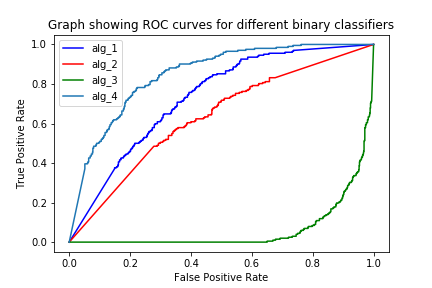
\includegraphics[width = 1.0\textwidth]{q4_c.png}
From the graph we can see that alg\_3 has worse than random performance. The only way to improve performance without retraining the model is by reversing the polarity for the outputs. This will effectively flip the ROC curve so it performs better than random.

\end{answerbox}



\end{subquestion}

\end{question}







\end{document}